\subsection[Scenariusz (Kacper Połom)]{Scenariusz} \label{sce:klawiatura}
Test polega na zdalnym wprowadzeniu dowolnej sekwencji klawiszy w systemie komputerowym. Oczekiwanym rezultatem jest odebranie danych przez system w taki sposób jakby wprowadzał je faktyczny użytkownik.
\subsubsection[Aktorzy]{Aktorzy}
\begin{itemize}
    \item Pentester - osoba przeprowadzająca test bezpieczeństwa systemu komputerowego za pomocą dedykowanego systemu
    \item Środowisko testowe (ST) - podsystem, monitoruje aktywne urządzenia wykonujące, odpowiada za komunikację między komponentami \textit{BSc-pentestera}
    \item Urządzenie wykonujące - niewielkie urządzenie oparte o platformę Raspberry Pi Zero W, podłączone za pomocą portu USB do testowanego systemu
    \item Testowany system - system komputerowy pracujący pod kontrolą systemu \textit{Windows 10}, użytkownik nie posiada uprawnień administratora
\end{itemize}
\subsubsection[Założenia początkowe]{Założenia początkowe}
Prawidłowa realizacja scenariusza wymaga, aby urządzenie wykonujące było podłączone przez port USB do testowanego systemu. Powinno ono posiadać własne połączenie z internetem. Testowany system komputerowy musi być włączony, żeby mógł dostarczyć zasilanie urządzeniu oraz odebrać od niego dane.
\subsubsection[Przebieg]{Przebieg}
Urządzenie wykonujące po otrzymaniu zasilania uruchamia skrypt, który odpowiada za komunikację z środowiskiem testowym i obsługę komunikacji przy użyciu USB.
Urządzenie rejestruje swoją obecność w ST.
Pentester przy pomocy dedykowanego panelu wskazuje urządzenie oraz wysyła do niego ładunek - wskazaną sekwencję klawiszy.
ST rozróżnia testowane systemy na podstawie zgłoszonych identyfikatorów. W tym samym czasie może być testowanych wiele systemów komputerowych.
Po otrzymaniu wiadomości z ładunkiem urządzenie wykonujące realizuje komunikację przez port USB i wysyła informacje o wciśnięciu kolejnych klawiszy. Przykładowym efektem takich działań może być uruchomienie wiersza poleceń oraz wprowadzenie skryptu powłoki, co można zaklasyfikować jako zdalne wykonanie kodu. Odstępy czasowe pomiędzy symulowaniem wciśnięcia kolejnych klawiszy są na tyle małe, że proces jest praktycznie niezauważalny dla użytkownika.
\begin{figure}[H]
    \centering
    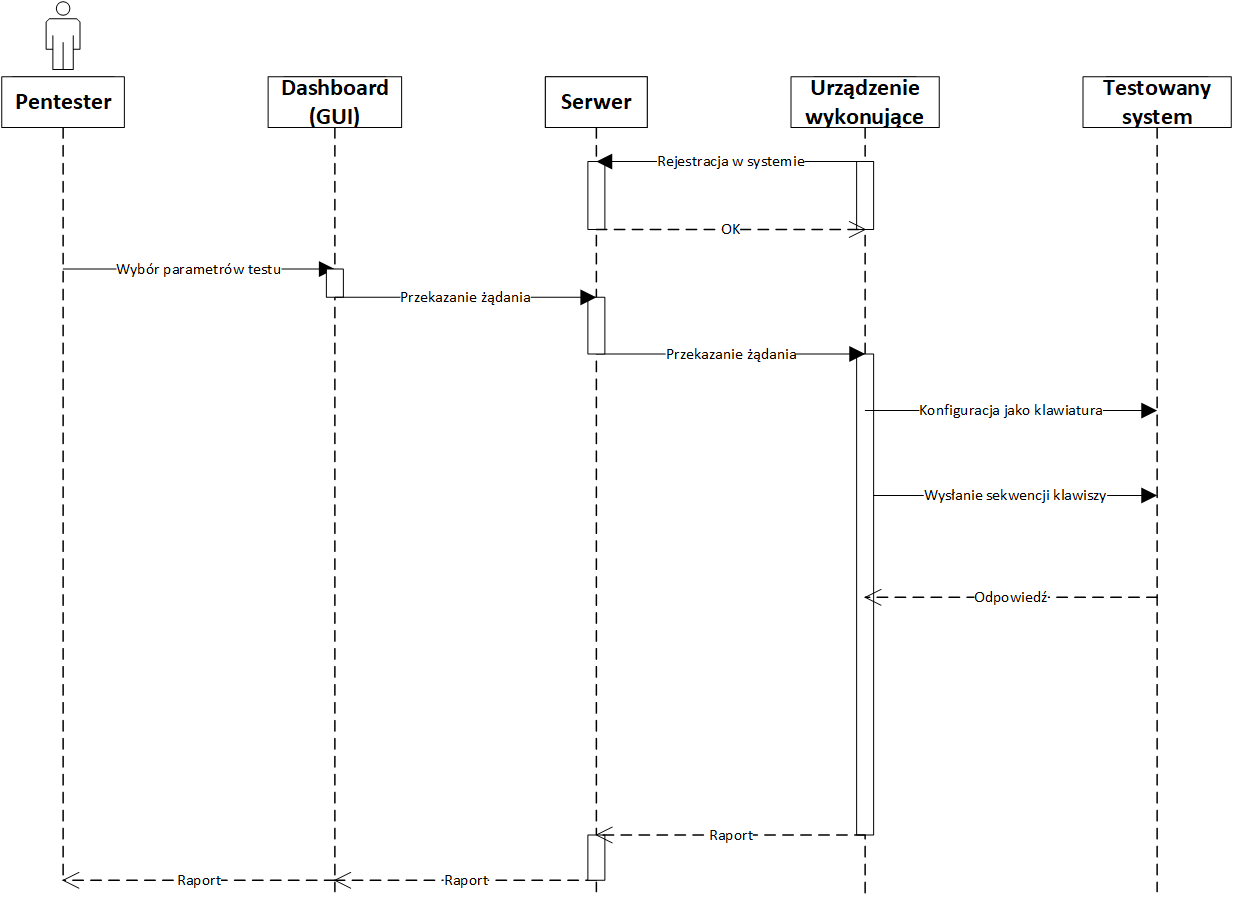
\includegraphics[width=\textwidth]{intKlaw}
    \caption{Diagram interakcji dot. testu symulowania działania klawiatury}
    \label{fig:klawiatura}  
\end{figure}